\section{Entwicklung}

Im Rahmen dieses Software-Projekts sollten wir eine Chrome-Extension entwickeln, die das Ticketsystem der Firma Projektron um KI-Funktionen erweitert. Dazu sollten wir einerseits ein lokales Modell (on-device) und ein externes Modell verwenden.

Wir haben Gemini Nano als lokales und Llama-3.3 als externes Modell verwendet.

\subsection{Gemini Nano}

Gemini Nano ist ein von Google entwickeltes Sprachmodell \cite{gemini-nano}. Der Hauptzweck von Gemini Nano ist es, KI Funktionen clientseitig ausführen zu können, ohne dafür jedesmal ein Sprachmodell herunterladen zu müssen. Dazu wurde Gemini Nano direkt in Chrome Canary integriert. \cite{gemini-nano-build-in-ai}

Aktuell befinden sich Gemini Nano und die dazugehörige API in einer Testphase. In diesem Zustand können und haben sich \footnote{Wie wir mehrfach während der Entwicklung unseres Plugins feststellen mussten} deren Funktionen ständig geändert. \cite{gemini-nano-build-in-ai}

Die Gemini API ist in verschiedene Task API's aufgeteilt. Aktuell sind dies \cite{gemini-nano-apis}:
\begin{itemize}
    \item LanguageDetection
    \item Translation
    \item Summary
    \item Writer + Rewriter
    \item PromptApi \footnote{Unser Plugin stützt sich letzlich auf die PromptApi, auch wenn wir zwischendurch die anderen API's ausprobiert haben.}
\end{itemize} 

\subsection{Dokumentation von Gemini Nano}

Um die oben genannten API's nutzen zu können sollte man dem Origin Trial beiteten. Dies ging über \cite{gemini-nano-origin-trial}. Hier erhiehlten wir die jeweils neuesten Informationen via Email. Dies war notwendig, da die eigentliche Dokumentation \cite{old-doku-language-detection-api, old-doku-translation-api,old-doku-summarization-api,old-doku-writer-api,old-doku-prompt-api} seit längerer Zeit nicht mehr aktuell ist (Stand 04.02.2025). Inzwischen gibt es zwar über \cite{gemini-nano-build-in-ai} eine neue öffentlich zugängliche Dokumentation, allerdings ist diese ebenfalls nicht vollständig.

\subsection{Crome Canary}

Chrome Canary ist die experimentelle Version von Googles Chrome Browser und bietet die Möglichkeit, die neuesten Funktionen zu testen. Canary kann als eine Art Labor betrachtet werden, in dem neue Ideen und Features ausprobiert werden, bevor sie in die endgültige Version von Chrome aufgenommen werden. Diese Vorabversion wird täglich aktualisiert, wodurch die neuesten Entwicklungen stets verfolgt werden können. Da es sich jedoch um eine experimentelle Version handelt, kann es vorkommen, dass Canary instabil ist oder Fehler aufweist \cite{chrome-canary}.

Zum Zeitpunkt der Entwicklung unserer Extension war Chrome Canary die einzige Möglichkeit Gemini Nano zu benutzen.

\subsection{Notwendige Voraussetzungen für Gemini Nano}

Gemini Nano ist unter Windows (10, 11) und unter MacOs (>=13) verfügbar, sofern man mindestens 22 GB freien Speicher hat, über eine GPU verfügt und >= 6 GB VideoRAM hat.

Um Gemini Nano in Chrome Canary nutzen zu können müssen dann mehrere Flags gesetzt werden. Dazu gibt man in der Adresszeile \texttt{chrome://flags} ein. Dort müssen dann folgende Flags gesetzt werden:
\begin{itemize}
    \item Enables optimization guide on device --> \emph{Enabled BypassPerfRequirement}
    \item Text Safety Classifier \footnote{Wenn der Text Safety Classifier nicht ausgeschaltet ist, weigert sich Gemini Nano Texte zu verarbeiten, die nicht in Englsich sind.} --> \emph{Disabled}
    \item Language detection web platform API --> \emph{Enabled}
    \item Experimental translation API --> \emph{Enabled without language pack limit}
    \item Summarization API for Gemini Nano --> \emph{Enabled}
    \item Writer API for Gemini Nano --> \emph{Enabled}
    \item Rewriter API for Gemini Nano --> \emph{Enabled}
    \item Prompt API for Gemini Nano --> \emph{Enabled}
\end{itemize}

Desweiteren sollte man danach in der Adresszeile \texttt{chrome://components/} eingeben und dann \emph{Optimization Guide On Device Model} suchen und aktualisieren.

Um zu testen, ob alles korrekt eingestellt ist und ob man die notwendigen Voraussetzungen erfüllt kann man nun in der Console  des Chrome Browsers \footnote{auf einem Mac: \texttt{Darstellung --> Entwickler --> Java-Script-Konsole}} folgendes eintippen: \texttt{await self.ai.languageModel.availability()} falls man nun \texttt{after-download} oder \texttt{available} als Antwort erhält, kann man Gemini Nano prinzipiell verwenden. Sollte man jedoch \texttt{no} als Antwort bekommen, so wird der verwendete Computer nie in der Lage sein Gemini Nano auszuführen.

\subsection{Chrome Extensions}

Chrome-Extensions \cite{chrome-extensions} sind kleine Softwareprogramme, die die Funktionalität des Google Chrome-Browsers erweitern und an die individuellen Bedürfnisse des Nutzers anpassen. Sie stellen eine Bereicherung des Browser-Erlebnisses dar, indem sie zusätzliche Funktionen implementieren, bestehende modifizieren oder repetitive Aufgaben automatisieren.

Chrome-Extensions basieren auf Webtechnologien wie HTML, CSS und JavaScript. Somit sind sie prinzipiell in jedem Texteditor erstellbar.

\subsection{TypeScript}

Typescript (TS) ist eine von Microsoft entwickelte Erweiterung von JavaScript (JS). \cite{typescript}

TS wird zu JS convertiert, wodurch der geschriebene Code in nahezu jedem Browser läuft. \cite{typescript}

TS erweitert JS durch ein Typsystem in dem unter anderem Interfaces und Klassen beschrieben werden können. Dadurch reduzieren sich die möglichen Fehlerquellen enorm, da der TS-Compiler einfache Typ-Überprüfungen vollziehen kann. Desweiteren ist dadurch auch eine bessere Integration mit IDE's wie zum Beispiel VSCode gegeben. \cite{typescript}

TS ist dabei so entworfen worden, dass jeder gültige JS-Code auch gültiger TS-Code ist. Es ist also möglich ein bestehendes JS-Projekt ohne weiteres auf TS umzustellen. Anschließend kann man, wenn man möchte, den vorhandenen Code zu TS convertieren. \cite{typescript} \cite{ts-doku} Dabei hilft ein Feature von TS. Die so genannte tsconfig.json Datei enthält Einstellungen für den TS-Compiler um beispielsweise erweitertes ErrorChecking zu ermöglichen. \cite{tsconfig}

\subsection{Wie haben wir Typescript genutzt?}

Aufgrund der vielen Vorteile von TS haben wir unsere Chrome Extension direkt und vollständig (100 \%) in TS geschrieben.

Außerdem haben wir die tsconfig.json Datei so eingestellt, dass der TS-Compiler maximal streng vorgeht. Dies bedeutet, dass wir so viele Warnungen und Vorschläge vom Compiler bekommen möchten, wie irgend möglich. Außerdem wurde eingestellt, dass jede Warnung als Fehler zu interpretieren ist und zum Abbruch führt. Für weitere Informationen zur tsconfig.json kann man auf der offiziellen Webseite \cite{tsconfig} nachsehen .

\subsection{Architektur}

\begin{figure}[htbp]
    \centering
    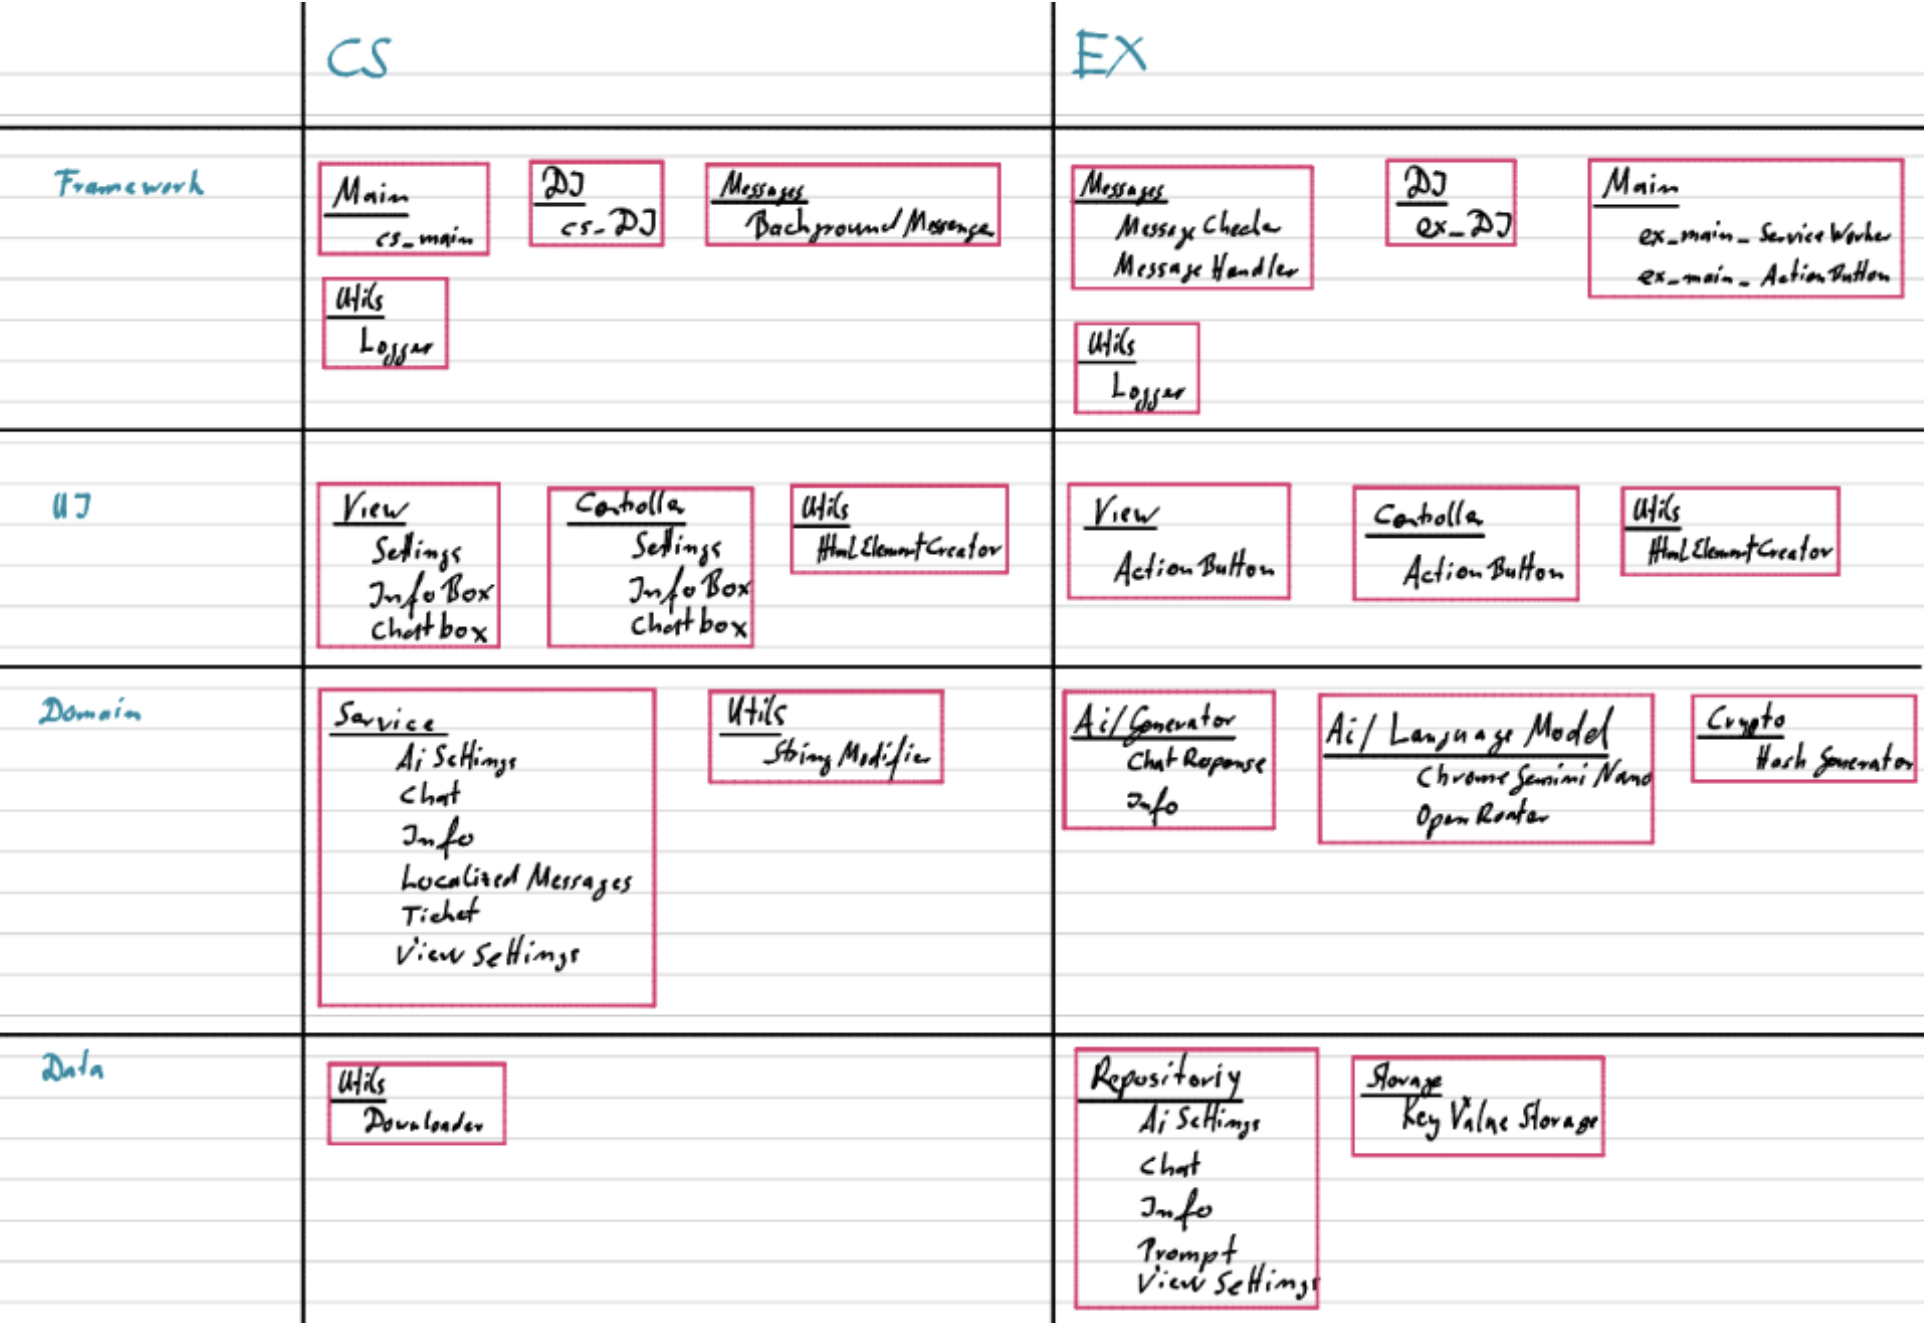
\includegraphics[width=1\textwidth]{img/Architektur.png}
    \caption{Architektur}
    \label{fig:Architektur}
  \end{figure}
